\documentclass[11pt]{article}
\usepackage[T1]{fontenc}
\usepackage{lmodern}
\usepackage[margin=1in]{geometry}
\usepackage{amsmath,amssymb,amsthm,mathtools}
\usepackage{microtype}
\usepackage{enumitem}
\usepackage{tikz}
\usetikzlibrary{arrows.meta}
\usepackage[colorlinks=true,linkcolor=blue,citecolor=blue,urlcolor=blue]{hyperref}
\usepackage[capitalise,noabbrev]{cleveref}
\hypersetup{pdftitle={One Rational Matrix Hitting Point for Noncommutative Formulas},pdfauthor={OpenAI}}
\newtheorem{theorem}{Theorem}[section]
\newtheorem{lemma}[theorem]{Lemma}
\newtheorem{proposition}[theorem]{Proposition}
\newtheorem{corollary}[theorem]{Corollary}
\theoremstyle{definition}
\newtheorem{definition}[theorem]{Definition}
\newtheorem{remark}[theorem]{Remark}
\DeclareMathOperator{\ord}{ord}
\DeclareMathOperator{\Mat}{Mat}
\DeclareMathOperator{\GL}{GL}
\newcommand{\Q}{\mathbb{Q}}
\newcommand{\C}{\mathbb{C}}
\title{One Rational Matrix Hitting Point\\for Noncommutative Formulas}
\author{OpenAI}
\date{September 24, 2026}
\begin{document}
\maketitle
\begin{abstract}
We construct, in deterministic polynomial bit time, one tuple of rational
matrices that detects every nonzero polynomial computed by a noncommutative
division-free formula of a prescribed size. The matrices have dimension $O(ns^2)$ for
$n$ variables and formula size $s$, and the same tuple works over every
field of characteristic zero.
\end{abstract}
\tableofcontents
\section{Introduction}
\label{sec:introduction}

Polynomial identity testing asks whether an arithmetic expression computes
the zero polynomial. We study this question for noncommuting variables when
the expression is accessible through matrix evaluations. The aim is to choose
the evaluation matrices before seeing the expression or any of its coefficients.

Let $F\langle x_1,\ldots,x_n\rangle$ be the free associative polynomial algebra
over a field $F$. A \emph{noncommutative formula} is a rooted tree whose leaves
are variables or scalars in $F$, and whose internal gates have two inputs and
are labelled $+$ or $\times$. The two inputs to each multiplication gate are
ordered. Its \emph{size} counts all gates, including the leaves. Write
$\mathsf{Form}_{n,s}(F)$ for the polynomials computed by formulas of size at
most $s$ in $n$ variables.

For a tuple $\mathbf T=(T_1,\ldots,T_n)\in\Mat_d(F)^n$, the value
$f(\mathbf T)$ is the usual ordered matrix evaluation; a scalar $a\in F$
acts as $aI_d$. A \emph{hitting point} for a class of polynomials is one tuple
on which every nonzero member of the class has nonzero matrix value.
More generally, a hitting set allows several tuples and requires a nonzero
value on at least one of them.

\begin{theorem}\label{thm:main}
There is a deterministic algorithm which, given integers $n,s\ge1$,
constructs a tuple
\[
 \mathbf T_{n,s}\in\Mat_d(\Q)^n,
 \qquad d\le 2ns^2,
\]
in time polynomial in $n,s$, measured in bit operations. The numerators and
denominators of its entries have bit length
$O(\log(ns+1)+ns^2\log(n+1))$.
For every field $F$ of characteristic zero and every
$0\ne f\in\mathsf{Form}_{n,s}(F)$,
\[
 f(\mathbf T_{n,s})\ne0,
\]
where the tuple is viewed over $F$ through the canonical embedding
$\Q\hookrightarrow F$. The construction uses $d=2ns^2$ when $ns\ge2$
and $d=1$ when $n=s=1$.
\end{theorem}

Thus a single exact matrix-evaluation query decides whether a polynomial
promised to lie in $\mathsf{Form}_{n,s}(F)$ is zero. The bit-time statement
concerns construction of the rational tuple. Evaluation over an arbitrary
field is understood as an exact oracle operation; no encoding or bit-cost
assumption on arbitrary elements of $F$ is needed. In particular, the singleton
set $\{\mathbf T_{n,s}\}$ gives a positive solution to the polynomial-size
rational-matrix hitting-set problem for characteristic-zero formulas.

\subsection{Context and scope}

An \emph{acyclic algebraic branching program} is a directed acyclic graph
with a designated source and sink, and with affine-linear edge labels
over the coefficient field. Its output is the sum of the ordered products
of edge labels along source-to-sink paths; here its size is the number
of vertices. Formulas admit such path representations of linear size.

Linear algebra has long played a central role in noncommutative complexity.
Nisan characterized layered homogeneous algebraic branching-program complexity by
ranks of coefficient matrices \cite[Theorem~1]{Nisan1991}.
Raz and Shpilka gave deterministic polynomial-time identity tests for
noncommutative formulas and algebraic branching programs
\cite[Theorems~4 and~5]{RazShpilka2005}. These algorithms use the internal structure
of the input, which is the white-box model. In the black-box model,
Bogdanov and Wee gave a randomized matrix-evaluation identity test with
one-sided error and running time polynomial in a supplied degree bound
and the other input parameters
\cite[Theorem~4.2]{BogdanovWee2005}.
Forbes and Shpilka constructed deterministic
quasipolynomial-size matrix hitting sets for noncommutative algebraic branching
programs over sufficiently large fields
\cite[Corollary~4.7]{ForbesShpilka2013}, and hence for formulas.
Their field-size condition is automatic in characteristic zero.

Arvind, Chatterjee and Mukhopadhyay obtained quasipolynomial black-box
tests over $\Q$ for rational formulas of inversion height two
\cite[Theorem~1.1]{ArvindChatterjeeMukhopadhyay2022}, and subsequently for
unrestricted noncommutative rational formulas
\cite[Theorem~2 and Corollary~3]{ArvindChatterjeeMukhopadhyay2026}.
Such formulas may have inverse gates, and evaluation requires each inverse
operand to be invertible. A separate manuscript
\cite[Theorem~1.1]{OpenAIRationalFormulas2026} constructs polynomial-size
rational matrix hitting lists for formulas over $\Q$ with a nonempty
rational matrix evaluation domain. Whenever such a formula is nonzero
on its domain, the list contains a defined evaluation with invertible
value, without a bound on inverse nesting or rational constant heights.
Here the single tuple works over every characteristic-zero coefficient
field for division-free formulas, whose matrix evaluations are everywhere
defined.

Two recent results treat different size restrictions. Lakhani and Mukhopadhyay
construct one integer matrix tuple for sparse noncommutative polynomials
over every characteristic-zero field, with polynomial construction time
and dimension equal to the sparsity bound, without a degree restriction
\cite[Theorem~2.1 and Remark~2.6]{LakhaniMukhopadhyay2026}.
Formula size can be much smaller than sparsity:
the ordered product of $k$ copies of $x_1+x_2$ has $4k-1$ gates and $2^k$
monomials. Lakhani and Saxena obtain randomized black-box tests for homogeneous
noncommutative circuits of constant depth
\cite[Theorem~1]{LakhaniSaxena2026}. Theorem~\ref{thm:main} is deterministic
and imposes no depth or homogeneity restriction on a formula.

The essential quantitative assertion is that matrix dimension, rational entry
length, and construction bit time are all polynomial in formula size and
the number of variables. For polynomials, a finite matrix hitting set can
always be combined into one tuple by taking block-diagonal sums, but the
resulting dimension is the sum of the dimensions in the set.
The construction here gives the polynomial
bounds directly. The formula model is used to obtain a small acyclic path
representation. In fact, Proposition~\ref{prop:path-programs} applies the
same construction to the algebraic branching programs defined above,
with matrix dimension $(n-1)\binom m2+m$ for $m$ vertices.
Thus the path-program consequence also improves the preceding
quasipolynomial hitting-set bound in characteristic zero.
No bound for arbitrary shared circuits is asserted.

\subsection{Proof idea}

The obstacle is that a small formula may contain exponentially many words
after expansion. We retain these words through a faithful encoding, and
bound the necessary truncation using a small representation of the formula.
We encode words by iterated integrals in one variable. For a word $w=i_1\cdots i_k$ on
$\{1,\ldots,n\}$, write $x_w=x_{i_1}\cdots x_{i_k}$, with
$x_\epsilon=1$ for the empty word. Define
\[
 h_{\epsilon}(z)=1,
 \qquad
 h_{iw}(z)=\int_0^z\frac{h_w(t)}{t+i}\,dt,
\]
where $\epsilon$ is the empty word and integration is interpreted by formal
power series at zero. Section~\ref{sec:iterated-integrals} proves that the
$h_w$ are linearly independent over every characteristic-zero field. Over
$\C$, continuation around the distinct poles yields a triangular spanning
argument in a truncated free algebra. A nonzero rational coefficient minor
then transfers independence to every field in the theorem. These functions
belong to the classical theory of iterated integrals and hyperlogarithms
\cite{Chen1977}. Their independence is a special case of the stronger
differential-field theorem of Deneufch\^atel, Duchamp, Hoang Ngoc Minh and
Solomon \cite[Theorem~1]{DeneufchatelEtAl2011}; we include a direct proof
for the particular kernels used here. Its triangular monodromy argument
has a two-letter antecedent in Minh, Petitot and van der Hoeven
\cite[Section~5, Theorem~4]{MinhPetitotVanderHoeven1998}.

If $f_w$ denotes the coefficient of $x_w$ in $f$, put
$h_f=\sum_w f_wh_w$.
Section~\ref{sec:formula-systems} converts a size-$s$ formula into an acyclic
path representation with at most $2s$ states, using the standard formula-to-path
construction of Nisan \cite[Section~2, Lemma~1]{Nisan1991}, also presented
by Raz and Shpilka \cite[Section~2.1, Lemma~2, Step~1]{RazShpilka2005}.
It follows that $h_f=uGv$ for
constant vectors $u,v$ and an invertible formal matrix $G$ satisfying
\[
 G'=\left(\sum_{i=1}^n\frac{B_i}{z+i}\right)G.
\]
The matrices $B_i$ describe the formula and are used only in the proof.

The quantitative step is a uniform bound on vanishing at zero.
Moura's multiplicity estimate for rational differential systems
\cite{Moura2003}, also stated in \cite[Section~2, Theorem~1]{MouraHyperelliptic2003},
bounds the order of a nonzero scalar component $uGv$
of an $m$-dimensional system $G'=(P/q)G$, with $q(0)\ne0$,
$\deg q=n$ and $\deg P\le n-1$, by
$(n-1)\binom m2+m-1$. Section~\ref{sec:multiplicity} gives a self-contained
formal proof of this estimate over the characteristic-zero field in use.
It uses the formal Wronskian criterion
\cite{BostanDumas2010} and the minimum order of the maximal minors of
a matrix of derivative rows. This bound is independent of all coefficient
values and applies beyond the particular systems arising from formulas.

Finally, Section~\ref{sec:construction} realizes the integration operators
on the space of Taylor coefficients of degrees below $2ns^2$.
Their matrices have explicit rational entries. Linear independence makes
$h_f$ nonzero, and the order bound ensures that this finite truncation retains
a nonzero coefficient. That coefficient occurs in the first column of
$f(\mathbf T_{n,s})$.

For $ns\ge2$, write $\pi_d(a)$ for the column of the first $d=2ns^2$
Taylor coefficients of a series $a$, and put $e_0=\pi_d(1)$.
Figure~\ref{fig:proof-route} summarizes the argument for a nonzero
formula polynomial $f$, separating the generator from the
formula-dependent objects used to prove its guarantee.
\begin{figure}[ht]
\centering
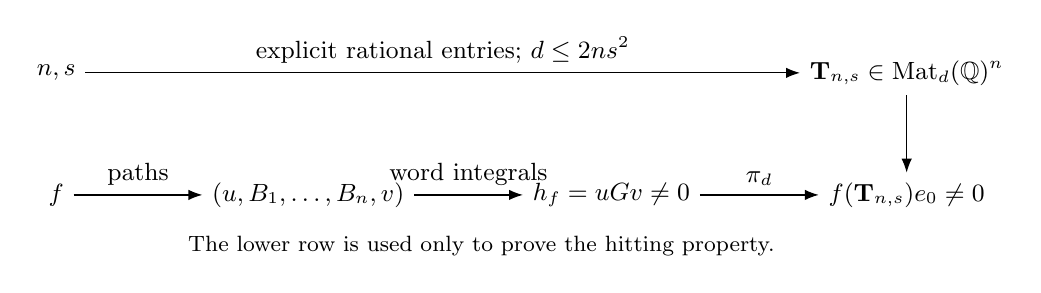
\begin{tikzpicture}[
  >=Latex,
  every node/.style={font=\small,align=center},
  every path/.style={line width=.45pt}
]
\node (bounds) at (0,1.55) {$n,s$};
\node (tuple) at (10.8,1.55) {$\mathbf T_{n,s}\in\Mat_d(\Q)^n$};
\draw[->] (bounds) -- node[above] {explicit rational entries; $d\le2ns^2$} (tuple);
\node (formula) at (0,0) {$f$};
\node (paths) at (3.2,0) {$(u,B_1,\ldots,B_n,v)$};
\node (series) at (7.05,0) {$h_f=uGv\ne0$};
\node (column) at (10.8,0) {$f(\mathbf T_{n,s})e_0\ne0$};
\draw[->] (formula) -- node[above] {paths} (paths);
\draw[->] (paths) -- node[above] {word integrals} (series);
\draw[->] (series) -- node[above] {$\pi_d$} (column);
\draw[->] (tuple) -- (column);
\node[font=\footnotesize] at (5.4,-.65)
  {The lower row is used only to prove the hitting property.};
\end{tikzpicture}

\caption{The construction for $ns\ge2$. The generator uses only the size bounds.
The correctness argument
associates a differential system to each possible input formula. Independence
makes its scalar output nonzero, and the multiplicity bound ensures that
the retained Taylor coefficients include a nonzero entry.}
\label{fig:proof-route}
\end{figure}

\section{A faithful encoding by iterated integrals}
\label{sec:iterated-integrals}

We first encode noncommutative polynomials as power series in one variable.
The encoding will preserve every nonzero polynomial; the remaining sections
will bound how many Taylor coefficients are needed for a small formula.

Fix an integer $n\geq 1$ and a field $F$ of characteristic zero.
For $i\in[n]=\{1,\ldots,n\}$, define an $F$-linear operator on $F[[z]]$ by
\begin{equation}
  \mathcal J_i(a)(z)=\int_0^z\frac{a(t)}{t+i}\,dt.
  \label{eq:integration-operator}
\end{equation}
Here integration means termwise formal integration with zero constant term:
expand $(t+i)^{-1}=\sum_{j\geq0}(-1)^j t^j/i^{j+1}$ first.
All denominators are nonzero in $F$.
For a nonzero series $a$, let $\operatorname{ord}_0 a$ denote the least
exponent with nonzero coefficient, and put $\operatorname{ord}_0 0=\infty$.
Then
\begin{equation}
  \operatorname{ord}_0\mathcal J_i(a)
  \geq \operatorname{ord}_0 a+1.
  \label{eq:integration-order}
\end{equation}

A word $w=i_1\cdots i_b$ on $[n]$ has length $|w|=b$;
the empty word is denoted by $\epsilon$.
Define the series $h_w\in\mathbb Q[[z]]$ recursively by
\begin{equation}
  h_\epsilon=1,\qquad h_{iw}=\mathcal J_i(h_w).
  \label{eq:word-series}
\end{equation}
We regard these series as elements of $F[[z]]$ through the canonical
embedding $\mathbb Q\hookrightarrow F$.
In particular, $\operatorname{ord}_0 h_w\geq |w|$.
Over $\mathbb C$, they are holomorphic germs at zero: the same recursion
uses ordinary integration on any disk of radius less than one.
These functions are classical iterated integrals, also called
hyperlogarithms; see Chen~\cite{Chen1977} for the general framework.
The following independence statement is a special case of
Deneufch\^atel et al.~\cite[Theorem~1]{DeneufchatelEtAl2011}.
Their criterion in fact gives independence over $F(z)$: no nonzero
$F$-linear combination of $1/(z+1),\ldots,1/(z+n)$ is the derivative
of a rational function, because such a derivative has zero residue
at every pole. We give a direct proof of the constant-coefficient
independence needed here.
We use a triangular monodromy argument, as in the two-letter case treated
by Minh, Petitot and van der Hoeven
\cite[Section~5, Theorem~4]{MinhPetitotVanderHoeven1998}.

\begin{lemma}[Linear independence of the word series]
\label{lem:word-independence}
For every integer $n\geq1$, every integer $D\geq0$, and every
characteristic-zero field $F$, the series
\[
  \{h_w: w\text{ is a word on }[n],\ |w|\leq D\}
\]
are linearly independent over $F$.
\end{lemma}

\begin{proof}
The case $D=0$ consists of the single series $1$.
Suppose $D\geq1$, and first work over $\mathbb C$.
Let $E_D$ be the complex algebra with basis $X_w$, $|w|\leq D$,
whose multiplication is concatenation of words, with products of length
greater than $D$ set equal to zero.
Its identity is $X_\epsilon=1$.
The span $\mathfrak m$ of the nonempty words is an ideal satisfying
$\mathfrak m^{D+1}=0$.
For one-letter words write $X_i=X_{(i)}$, and set
\[
  U(z)=\sum_{|w|\leq D}h_w(z)X_w.
\]
The recursion \eqref{eq:word-series} gives the left differential equation
\begin{equation}
  U'(z)=\left(\sum_{i=1}^n\frac{X_i}{z+i}\right)U(z),
  \qquad U(0)=1.
  \label{eq:word-differential-equation}
\end{equation}
This is a linear equation on the finite-dimensional vector space $E_D$,
with coefficients holomorphic on
$\Omega=\mathbb C\setminus\{-1,\ldots,-n\}$.
For this particular equation, local existence and uniqueness follow
directly by induction on word length: the derivative of a length-$b$
coefficient is determined by length-$(b-1)$ coefficients. On a disk
avoiding the poles, taking holomorphic primitives with prescribed initial
values therefore constructs the solution in $D$ steps.
A finite chain of overlapping disks continues it along any path in
$\Omega$, and uniqueness makes the solutions agree on overlaps.

For a loop $\gamma$ in $\Omega$ based at zero, let $Q_\gamma$ be the
value at zero after continuation around $\gamma$.
It belongs to $1+\mathfrak m$, since the constant coefficient of the
solution remains one.
Suppose that $\sum_{|w|\leq D}c_w h_w=0$ as a complex germ, and define
a complex-linear functional $\lambda:E_D\to\mathbb C$ by
$\lambda(X_w)=c_w$.
The germ $\lambda(U)$ is zero, and its continuation around every loop
is zero; hence $\lambda(Q_\gamma)=0$ for every $\gamma$.
It therefore suffices to prove that the loop values span $E_D$.

The order of multiplication matters here.
Along a fixed path, a solution with initial value $b\in E_D$ equals
the solution with initial value one multiplied by $b$ on the right.
Thus traversing $\gamma$ and then $\delta$ gives
$Q_\delta Q_\gamma$.
In particular, the set of loop values contains $1$, and every ordered
product of loop values is again a loop value.

Choose a based loop $\gamma_i$ with winding number one about $-i$
and zero about every other pole, and put $Q_i=Q_{\gamma_i}$.
One may take an access path from zero, a small positive circle about
$-i$, and the reversed access path. For the degree-one integrals the
two access paths cancel. Direct integration on the circle gives
$2\pi\sqrt{-1}$ for $dz/(z+i)$ and zero for $dz/(z+j)$ when $j\ne i$;
the latter also follows by integrating its convergent Taylor expansion
on the disk bounded by the circle.
Reducing \eqref{eq:word-differential-equation} modulo $\mathfrak m^2$
and integrating around this loop yields
\[
  Q_i=1+\tau X_i\pmod{\mathfrak m^2},
  \qquad \tau=2\pi\sqrt{-1}.
\]
For $w=i_1\cdots i_b$, define
\[
  C_w=(Q_{i_1}-1)\cdots(Q_{i_b}-1),
  \qquad C_\epsilon=1.
\]
Expanding the product shows that $C_w$ lies in the complex linear span
of the loop values.
It has no terms of word length less than $b$, and its length-$b$ part
is $\tau^b X_w$.
Consequently the family $\{C_w:|w|\leq D\}$ is a basis of $E_D$:
in a word basis ordered by length, its coefficient matrix is triangular
with nonzero diagonal entries $\tau^{|w|}$.
The loop values therefore span $E_D$, so $\lambda=0$.
This proves complex linear independence.

To pass to $F$, form the matrix whose columns are the Taylor
coefficients of the finitely many series $h_w$, $|w|\leq D$.
Every entry is rational.
The kernels over $\mathbb C$ of its successive finite row prefixes
form a descending sequence of subspaces of a fixed finite-dimensional
space.
Their intersection is zero by the complex independence just proved,
so some finite prefix has full column rank.
It therefore contains a square minor with nonzero rational determinant.
That determinant stays nonzero under $\mathbb Q\hookrightarrow F$,
which rules out every $F$-linear relation among the series.
This minor is used only to prove independence; the construction of
the hitting point does not compute it.
\end{proof}

For $w=i_1\cdots i_b$, write $x_w=x_{i_1}\cdots x_{i_b}$ and
$x_\epsilon=1$.
Given $f=\sum_w f_w x_w\in F\langle x_1,\ldots,x_n\rangle$, define
\begin{equation}
  h_f=\sum_w f_w h_w.
  \label{eq:polynomial-series}
\end{equation}
Lemma~\ref{lem:word-independence} says that the $F$-linear map
$f\mapsto h_f$ is injective.
It is not an algebra homomorphism into $F[[z]]$.
Instead, the ordered word $x_{i_1}\cdots x_{i_b}$ acts by the composition
$\mathcal J_{i_1}\cdots\mathcal J_{i_b}$, applied to $1$:
\begin{equation}
  h_f=f(\mathcal J_1,\ldots,\mathcal J_n)1.
  \label{eq:operator-evaluation}
\end{equation}
For example, when $n\ge2$, the commutator $x_1x_2-x_2x_1$ gives
\[
 h_{12}(z)-h_{21}(z)=-\frac{z^3}{24}+O(z^4).
\]
Thus the encoding retains word order, but cancellation can delay the first
nonzero coefficient beyond the word length. We next use formula size to
bound this delay uniformly.

\section{From formulas to differential systems}
\label{sec:formula-systems}

The word functions from Section~\ref{sec:iterated-integrals} turn a nonzero
polynomial $f=\sum_w f_wx_w$ into the nonzero series
$h_f=\sum_w f_wh_w$.  We now express this series as a scalar output of a
differential system whose dimension is at most twice the formula size.
This small system will control how late the first nonzero coefficient of
$h_f$ can occur. The underlying formula-to-path construction is due to
Nisan~\cite[Section~2, Lemma~1]{Nisan1991}; see also Raz and
Shpilka~\cite[Section~2.1, Lemma~2, Step~1]{RazShpilka2005}.

\begin{lemma}[Acyclic coefficient representation]
\label{lem:formula-representation}
Let $F$ be a field, and let $f\in F\langle x_1,\ldots,x_n\rangle$
be computed by a fan-in-two formula with at most $s$ gates, counting
leaves.  There are an integer $m\le 2s$, a row
$u\in F^{1\times m}$, a column $v\in F^{m\times1}$, and strictly
upper triangular matrices $B_1,\ldots,B_n\in F^{m\times m}$ such that
\begin{equation}
\label{eq:formula-representation}
 f_w=uB_wv\quad\text{for every word }w,
 \qquad
 B_{i_1\cdots i_k}=B_{i_1}\cdots B_{i_k},\quad B_\epsilon=I_m.
\end{equation}
In particular, $B_w=0$ whenever $|w|\ge m$.
\end{lemma}

\begin{proof}
Construct a directed acyclic graph for each subformula, with a designated
source having no incoming edges and a designated sink having no outgoing
edges.  Each edge is labeled either by a variable or by a scalar in $F$.
The label of a path is the ordered product of its edge labels.

A leaf gives two vertices joined by one edge with the leaf's label.
For a sum, take disjoint copies of the two child graphs, add a new source
and sink, and join the new source to both child sources and both child
sinks to the new sink by edges labeled $1$.  For an ordered product,
take disjoint child graphs and join the first child's sink to the second
child's source by an edge labeled $1$; retain the first source and the
second sink.  These operations preserve acyclicity and the stated
source and sink properties.  A path through a sum chooses one child,
whereas a path through a product traverses the first child and then the
second.  Induction therefore shows that the sum of source-to-sink path
labels is $f$.

If the formula has $L$ leaves and $a$ addition gates, the graph has
$m=2L+2a\le2s$ vertices: multiplication adds no vertex.  Order the
vertices topologically.  Let $E$ be the adjacency matrix of the scalar
edges, with their scalar weights, and let $N_i$ be the adjacency matrix
of the edges labeled $x_i$, with weight $1$.  In each adjacency matrix,
row $a$ and column $b$ record edges from $a$ to $b$; parallel-edge weights
are summed.  All these matrices are strictly upper triangular.  The matrix
\[
 Q=(I_m-E)^{-1}=I_m+E+\cdots+E^{m-1}
\]
records all paths consisting only of scalar edges, including the empty
path at each vertex.  Write $e_j$ for the $j$th standard column vector.
If $\sigma$ and $\rho$ are the source and sink,
every path with variable word $i_1\cdots i_k$ decomposes uniquely into
scalar subpaths separated by those $k$ variable edges.  Consequently
\[
 f_{i_1\cdots i_k}
 =e_\sigma^{\mathsf T}Q N_{i_1}Q\cdots N_{i_k}Qe_\rho,
 \qquad
 f_\epsilon=e_\sigma^{\mathsf T}Qe_\rho.
\]
Set
\[
 u=e_\sigma^{\mathsf T}Q,\qquad v=e_\rho,
 \qquad B_i=N_iQ.
\]
Then \eqref{eq:formula-representation} follows.  Multiplying a strictly
upper triangular matrix by an upper triangular matrix preserves strict
upper triangularity, so each $B_i$ has that property.  A product of $m$
strictly upper triangular $m\times m$ matrices is zero, proving the
last assertion.
\end{proof}

This construction allows arbitrary scalar leaves and constant terms.
Its size bound uses the formula tree: the child graphs represent
disjoint subtrees, so each gate is counted once.  The construction does
not enumerate the monomials of $f$.

\begin{proposition}[The system associated to a formula]
\label{prop:formula-system}
Let $F$ have characteristic zero, and let
$0\ne f\in F\langle x_1,\ldots,x_n\rangle$ have a formula of size at
most $s$.  There are $m\le2s$, a nonzero constant row $u$, a constant
column $v$, and an invertible matrix $G\in F[[z]]^{m\times m}$ such that
\begin{equation}
\label{eq:formula-system}
 G'=AG,\qquad G(0)=I_m,\qquad
 A(z)=\frac{P(z)}{q(z)},\qquad
 q(z)=\prod_{i=1}^n(z+i),\quad \deg P\le n-1,
\end{equation}
where $P$ is a polynomial matrix.  Moreover,
\begin{equation}
\label{eq:formula-output}
 h_f(z)=\sum_w f_wh_w(z)=uG(z)v\ne0.
\end{equation}
\end{proposition}

\begin{proof}
Take the representation from Lemma~\ref{lem:formula-representation}
and define the finite sum
\[
 G(z)=\sum_{|w|<m}B_wh_w(z),\qquad
 A(z)=\sum_{i=1}^n\frac{B_i}{z+i}.
\]
The empty word contributes $I_m$, and every other $h_w$ has zero
constant term.  Thus $G(0)=I_m$, which makes $G$ invertible over
$F[[z]]$.  The identity $h_{iw}'=h_w/(z+i)$ gives
\[
 G'
 =\sum_{i=1}^n\sum_{|w|<m-1}
       \frac{B_iB_wh_w}{z+i}
 =AG.
\]
The terms with $|w|=m-1$ added in the last equality vanish because
$B_iB_w=0$.  In particular the system acts on the \emph{left}, in
the same order as the letters of a word.

The denominator in \eqref{eq:formula-system} is nonzero at zero:
$q(0)=n!\ne0$.  Its numerator is
\[
 P(z)=\sum_{i=1}^n B_i\prod_{j\ne i}(z+j),
\]
whose entries have degree at most $n-1$.  Finally,
\eqref{eq:formula-representation} gives $uGv=h_f$.
This series is nonzero by Lemma~\ref{lem:word-independence}, since
$f\ne0$; in particular $u\ne0$.
\end{proof}

We have obtained a nonzero series $h_f$ inside a system of dimension at
most $2s$, with a denominator of degree $n$ and a regular expansion
point at zero.  The next section bounds its vanishing order using only
these parameters, uniformly in all scalar coefficients of the formula.

\section{A bound on the order of vanishing}
\label{sec:multiplicity}

The preceding representation turns a formula into a scalar component of a
rational differential system. A multiplicity estimate of
Moura~\cite{Moura2003} bounds how long such a component can vanish.
We give a self-contained formal proof of the required estimate,
valid directly over any field of characteristic zero.

For a nonzero series $b\in F[[z]]$, write $\operatorname{ord}_0 b$ for the
least exponent with nonzero coefficient, and put
$\operatorname{ord}_0 0=+\infty$.  For $b_1,\ldots,b_k\in F[[z]]$,
their \emph{Wronskian} is
\[
 W(b_1,\ldots,b_k)
 =\det\bigl(b_\ell^{(j)}\bigr)_{
       0\le j<k,\,1\le\ell\le k}.
\]
The proof of the formal power-series Wronskian criterion by
Bostan and Dumas~\cite[Theorem~2 and Lemmas~1--3]{BostanDumas2010}
uses a basis with distinct orders and a Vandermonde determinant.
We recall that argument, recording also the order of the Wronskian.

\begin{lemma}\label{lem:wronskian}
Let $F$ be a field of characteristic zero and let $V\subset F[[z]]$ be a
vector space of finite positive dimension $k$ over $F$.  There is a basis
$b_1,\ldots,b_k$ of $V$ with distinct orders
$0\le a_1<\cdots<a_k$.  For this basis,
\begin{equation}\label{eq:wronskian-order}
 \operatorname{ord}_0 W(b_1,\ldots,b_k)
 =\sum_{\ell=1}^k a_\ell-\binom{k}{2}.
\end{equation}
In particular, the Wronskian of any basis of $V$ is nonzero, its order
does not depend on the basis, and every nonzero member of $V$ has order
at most $a_k$.
\end{lemma}

\begin{proof}
Consider the decreasing filtration $V_r=V\cap z^rF[[z]]$ for $r\ge0$.
The coefficient of $z^r$ embeds $V_r/V_{r+1}$ into $F$, so each quotient
has dimension at most one.  Moreover, $\bigcap_r V_r=0$.  Since $V$ is
finite-dimensional, the filtration is eventually zero: otherwise its
dimensions would eventually stabilize at a positive value, and then the
subspaces themselves would stabilize, contradicting the zero
intersection.  Choosing a vector at each of the $k$ dimension drops
gives a basis with the asserted distinct orders.  A nonzero linear
combination has the order of its lowest-order basis term.

Write $b_\ell=\beta_\ell z^{a_\ell}+\cdots$, with
$\beta_\ell\ne0$.  Factoring $z^{a_\ell}$ from column $\ell$ and $z^{-j}$
from row $j$ in the Laurent-series field, the remaining constant
determinant is
\[
 \left(\prod_{\ell=1}^k\beta_\ell\right)
 \det\bigl((a_\ell)_j\bigr)_{j,\ell}
 =\left(\prod_{\ell=1}^k\beta_\ell\right)
   \prod_{r<\ell}(a_\ell-a_r).
\]
Here $(a)_0=1$ and $(a)_j=a(a-1)\cdots(a-j+1)$; these are monic
polynomials of successive degrees, so their determinant is the
Vandermonde determinant.  It is nonzero in characteristic zero.  The
factorization remains valid when $a_\ell<j$: the corresponding falling
factorial vanishes and the remaining entry is still a power series.
This proves \eqref{eq:wronskian-order}.  A change of basis over $F$
multiplies the Wronskian by the nonzero determinant of the constant
change-of-basis matrix, proving the remaining assertions.
\end{proof}

The bound below is the specialization of Moura's estimate to the present
degree assumptions. In its complex formulation, recalled in
\cite[Section~2, Theorem~1]{MouraHyperelliptic2003}, the bound is
$m-1+\binom m2(\sigma-2)$, where $\sigma$ is the sum of pole orders
of the matrix differential form $(P/q)\,dz$ on the projective line.
The finite poles contribute at most $n$, and infinity contributes at
most one. The case $P=0$ is immediate, since every solution is constant.
The argument below proves the stated bound formally and follows the
same derivative-row and Wronskian method.

\begin{theorem}[Multiplicity estimate of Moura]\label{thm:multiplicity}
Let $F$ be a field of characteristic zero, and let $n,m\ge1$.
Suppose that $q\in F[z]$ has degree $n$ and $q(0)\ne0$, that
$P\in\operatorname{Mat}_m(F[z])$ has entries of degree at most $n-1$,
and that
\[
 G\in\operatorname{GL}_m(F[[z]]),\qquad G'=(P/q)G.
\]
For a constant row $u\in F^{1\times m}$ and a constant column
$v\in F^{m\times1}$, if $y=uGv$ is nonzero, then
\begin{equation}\label{eq:multiplicity-bound}
 \operatorname{ord}_0 y\le(n-1)\binom{m}{2}+m-1.
\end{equation}
\end{theorem}

\begin{proof}
Put $h=uG$, and let $V$ be the $F$-span of its $m$ component series.
Since $y\ne0$, its dimension $k$ satisfies $1\le k\le m$.
We compare Wronskians of these components with minors of a rational
matrix whose numerator degrees are controlled.

Define rational rows
\[
 R_0=u,\qquad R_{j+1}=R_j'+R_jP/q.
\]
Then $h^{(j)}=R_jG$.  Writing $R_j=Z_j/q^j$, the recurrence becomes
\[
 Z_0=u,\qquad
 Z_{j+1}=qZ_j'-jq'Z_j+Z_jP.
\]
Induction shows that $Z_j$ is a polynomial row with entries of degree
at most $j(n-1)$.  This includes $n=1$, when every $Z_j$ is constant.
Every $R_j$ is regular at zero, because $q(0)\ne0$.

Let $B$ be the $k\times m$ matrix with rows
$R_0,\ldots,R_{k-1}$, and put $S=\binom{k}{2}$.
The rows of $BG$ are $h,h',\ldots,h^{(k-1)}$.
Some $k$ components of $h$ form a basis of $V$, so
Lemma~\ref{lem:wronskian} gives a nonzero $k\times k$ minor of $BG$.
Since $G$ is invertible, $B$ also has a nonzero $k\times k$ minor.
Every such minor has denominator $q^S$ and polynomial numerator of
degree at most $(n-1)S$.  As $q(0)\ne0$, the minimum order $\delta$
among the nonzero $k\times k$ minors of $B$ satisfies
\begin{equation}\label{eq:minor-order}
 0\le\delta\le(n-1)S.
\end{equation}

The minimum order of the $k\times k$ minors of $BG$ is also $\delta$.
Indeed, Cauchy--Binet expresses every such minor as an $F[[z]]$-linear
combination of the minors of $B$, so its order is at least $\delta$.
Applying the same argument to $B=(BG)G^{-1}$ gives the reverse
inequality, because $G^{-1}$ also has power-series entries.
Equivalently, multiplication by $G$ preserves the ideal generated by
these minors in $F[[z]]$.

A nonzero minor of $BG$ attaining this minimum is a Wronskian of $k$
components of $h$.  Those components are linearly independent over
$F$, and hence form a basis of $V$.  Replace them by a basis of distinct
orders $a_1<\cdots<a_k$ as in Lemma~\ref{lem:wronskian}.  Its Wronskian
still has order $\delta$, so
\[
 \delta=\sum_{j=1}^k\bigl(a_j-(j-1)\bigr).
\]
Every summand is nonnegative.  Since $y\in V$ is nonzero, the same
Lemma and \eqref{eq:minor-order} give
\[
 \operatorname{ord}_0 y\le a_k
 \le\delta+k-1
 \le(n-1)\binom{k}{2}+k-1
 \le(n-1)\binom{m}{2}+m-1.
\]
\end{proof}

For the formula systems of the preceding section,
$q(z)=\prod_{i=1}^n(z+i)$ and $G(0)=I$, so every hypothesis of
Theorem~\ref{thm:multiplicity} holds.  Word-series independence makes
$uGv$ nonzero for a nonzero formula polynomial; the theorem bounds the
number of Taylor coefficients needed to detect it.  We now realize
these coefficients by finite rational matrices.

\section{The rational hitting point}
\label{sec:construction}

We now turn the integration operators into finite matrices and prove
Theorem~\ref{thm:main}. The hitting matrices depend only on the size parameters;
the representation of a polynomial is used to prove that they detect it.

\subsection{Taylor coefficients as a matrix space}

For $d\ge1$ and a characteristic-zero field $F$, let
\[
 \pi_d:F[[z]]\longrightarrow F^d,
 \qquad
 \pi_d\left(\sum_{r\ge0}a_rz^r\right)=(a_0,\ldots,a_{d-1})^{\mathsf T}.
\]
This identifies $F[[z]]/(z^d)$ with the column space having ordered basis
$1,z,\ldots,z^{d-1}$. The operator
$\mathcal J_i(a)=\int_0^z a(t)/(t+i)\,dt$ increases vanishing order, so it
induces a linear map on this quotient. Its matrix $T_i\in\Mat_d(\Q)$ is
\begin{equation}\label{eq:explicit-matrices}
 (T_i)_{r,q}=
 \begin{cases}
 \displaystyle\frac{(-1)^{r-q-1}}{r\,i^{\,r-q}},&0\le q<r<d,\\[4pt]
 0,&0\le r\le q<d.
 \end{cases}
\end{equation}
Indeed,
\[
 \frac1{z+i}=\sum_{a\ge0}\frac{(-1)^az^a}{i^{a+1}},
 \qquad
 \mathcal J_i(z^q)
 =\sum_{r>q}\frac{(-1)^{r-q-1}}{r\,i^{r-q}}z^r.
\]
Every denominator in the nonzero case is nonzero, since $r\ge1$ and $i\ge1$.
Discarding terms of degree at least $d$ before applying $\mathcal J_i$
does not change any retained coefficient. Thus, for every $a\in F[[z]]$,
\begin{equation}\label{eq:jet-intertwining}
 \pi_d(\mathcal J_i a)=T_i\pi_d(a).
\end{equation}

Let $e_0=\pi_d(1)$. For a word $w=i_1\cdots i_k$, repeated application of
\eqref{eq:jet-intertwining} gives
\[
 T_{i_1}\cdots T_{i_k}e_0=\pi_d(h_w).
\]
The rightmost matrix acts first, exactly as in
$h_w=\mathcal J_{i_1}\cdots\mathcal J_{i_k}(1)$.
For the empty word both products are identities. Consequently, for every
$f=\sum_w f_wx_w\in F\langle x_1,\ldots,x_n\rangle$,
\begin{equation}\label{eq:first-column}
 f(T_1,\ldots,T_n)e_0=\pi_d(h_f).
\end{equation}
This identity also accounts for constant terms, since a scalar is evaluated
as a scalar matrix.

\subsection{Detection and construction cost}

Suppose first that $ns\ge2$, and set $d=2ns^2$ in
\eqref{eq:explicit-matrices}. Let $F$ have characteristic zero, and let
$f\in\mathsf{Form}_{n,s}(F)$ be nonzero. By
Lemma~\ref{lem:word-independence}, its series $h_f$ is nonzero.
Proposition~\ref{prop:formula-system} represents this series as $uGv$
in a system of dimension $m\le2s$ satisfying the hypotheses of
Theorem~\ref{thm:multiplicity}. Hence
\begin{align*}
 \ord_0h_f
 &\le (n-1)\binom m2+m-1\\
 &\le (n-1)\binom{2s}{2}+2s-1
 \le 2ns^2-1=d-1.
\end{align*}
The last inequality follows from
\[
 (2ns^2-1)-\left((n-1)\binom{2s}{2}+2s-1\right)
 =s(2s+n-3)\ge0.
\]
Therefore $\pi_d(h_f)\ne0$. Equation~\eqref{eq:first-column} supplies a
nonzero first column of $f(T_1,\ldots,T_n)$, proving detection.

When $n=s=1$, a formula of size at most one is a single scalar or variable
leaf. The one-by-one tuple $T_1=[1]$ detects every nonzero polynomial in this
class. This gives dimension one in the remaining case.

For completeness, we give the bit cost of constructing the tuple.
With $d=2ns^2$, put
\[
 B=3+\lceil\log_2(d+1)\rceil
       +d\lceil\log_2(n+1)\rceil.
\]
Every nonzero entry in \eqref{eq:explicit-matrices} has numerator $1$ or $-1$
and positive denominator $r i^{r-q}$, of bit length at most $B$.
These fractions are already in lowest terms. For each $i$, precompute
$i,i^2,\ldots,i^{d-1}$ by repeated multiplication, then form each denominator
by multiplying one of these powers by $r$. There are $O(nd^2)$ such integer
operations on $O(B)$-bit integers. Schoolbook multiplication gives total
bit cost $O(nd^2B^2)$, with output length $O(nd^2B)$.
Both bounds are polynomial in $n,s$, and the stated entry bound in
Theorem~\ref{thm:main} follows by substituting $d=2ns^2$.
The branch $n=s=1$ has constant output and cost.
This completes the proof of Theorem~\ref{thm:main}.

\subsection{Acyclic path programs}

The formula-to-path conversion is the only step that uses the tree model.
The remaining argument applies to any strictly upper triangular coefficient
representation, with its number of states in place of the formula-size bound.

\begin{samepage}
\begin{proposition}
For every pair of integers $n,m\ge1$,\label{prop:path-programs}\label{rem:path-programs}
the matrices in
\eqref{eq:explicit-matrices}, with
\[
 d=(n-1)\binom m2+m,
\]
form a rational hitting point for the following class over every
characteristic-zero field $F$: nonzero polynomials
$f=\sum_w f_wx_w\in F\langle x_1,\ldots,x_n\rangle$ whose coefficients admit
a representation $f_w=uB_wv$, where $u\in F^{1\times m}$,
$v\in F^{m\times1}$, and $B_1,\ldots,B_n\in\Mat_m(F)$ are strictly upper
triangular. The tuple depends only on $n,m$ and can be constructed in time
polynomial in $n,m$, measured in bit operations.
\end{proposition}
\end{samepage}

\begin{proof}
For such a representation, define
$G=\sum_{|w|<m}B_wh_w$. Strict upper triangularity makes all longer products
zero. As in Proposition~\ref{prop:formula-system}, this gives
$G(0)=I_m$ and
\[
 G'=\left(\sum_{i=1}^n\frac{B_i}{z+i}\right)G,
 \qquad uGv=h_f.
\]
Thus $G$ is invertible over $F[[z]]$, and the system has the denominator
and numerator degrees in \eqref{eq:formula-system}.
The series $h_f$ is nonzero by Lemma~\ref{lem:word-independence}.
Theorem~\ref{thm:multiplicity} gives $\ord_0 h_f\le d-1$, so
\eqref{eq:first-column} proves detection. The preceding entry and output
cost calculation applies to this value of $d$ as well, and $d$ is polynomial
in $n,m$.
\end{proof}

In particular, an acyclic path program on $m$ vertices with scalar- or
variable-labelled edges has such a representation by the scalar-edge
elimination in Lemma~\ref{lem:formula-representation}. The same vertex bound
holds for the affine-linear edge labels allowed in an algebraic branching
program. To see this, order its vertices topologically and write each edge
label as $c_0+\sum_{i=1}^n c_i x_i$. Let $E_{ab}$ sum the coefficients $c_0$
over edges from $a$ to $b$, and let $(N_i)_{ab}$ sum their coefficients $c_i$.
Both $E$ and each $N_i$ are strictly upper triangular. Expanding the ordered
path products and putting $Q=(I_m-E)^{-1}$ gives, for source $\sigma$ and
sink $\rho$,
\[
 f_{i_1\cdots i_k}
 =e_\sigma^{\mathsf T}Q N_{i_1}Q\cdots N_{i_k}Qe_\rho.
\]
For the empty word the right side is $e_\sigma^{\mathsf T}Qe_\rho$.
Thus $u=e_\sigma^{\mathsf T}Q$, $B_i=N_iQ$, and $v=e_\rho$ give the
required representation without adding vertices.

{\small
\bibliographystyle{plain}
\bibliography{references}
}
\end{document}
